\documentclass{beamer}
\usetheme{default}

\usepackage[dutch]{babel}
\usepackage{graphicx}
\usepackage{pdfpages}
\usepackage{hyperref}

%Information to be included in the title page:
\title{Activation Records (AR)}
\author{Tobias Lamote \& Tim Robensyn}
\date{9 november 2023}

\begin{document}

% Verwelkom iedereen
\frame{\titlepage}

\begin{frame}{Inhoudstafel}
	\begin{itemize}
	    \item Herhaling
	    \item Parameter passing
	    \item Tail call optimization
	    \item Stack smashing
	    \item Demo met \texttt{gdb}
	    \item Nested functions
	    \item Continuations
	    \item Examenvragen
	\end{itemize}
\end{frame}

% Korte herhaling: procedure (pre-call, prologue, epilogue, post-call)?
% Situeer AR in de compiler:
%   - doel AR: definieer contract tussen aparte procedures
%   - machine-dependent
%   - input is AST
%   - output is frames, maar nog niet helemaal (register allocator volgt nog!)
%   - verwachting dat publiek al veel kent van de stack (CASS voor ingenieurs, SOCKS voor informatici)
\begin{frame}{Situering}
    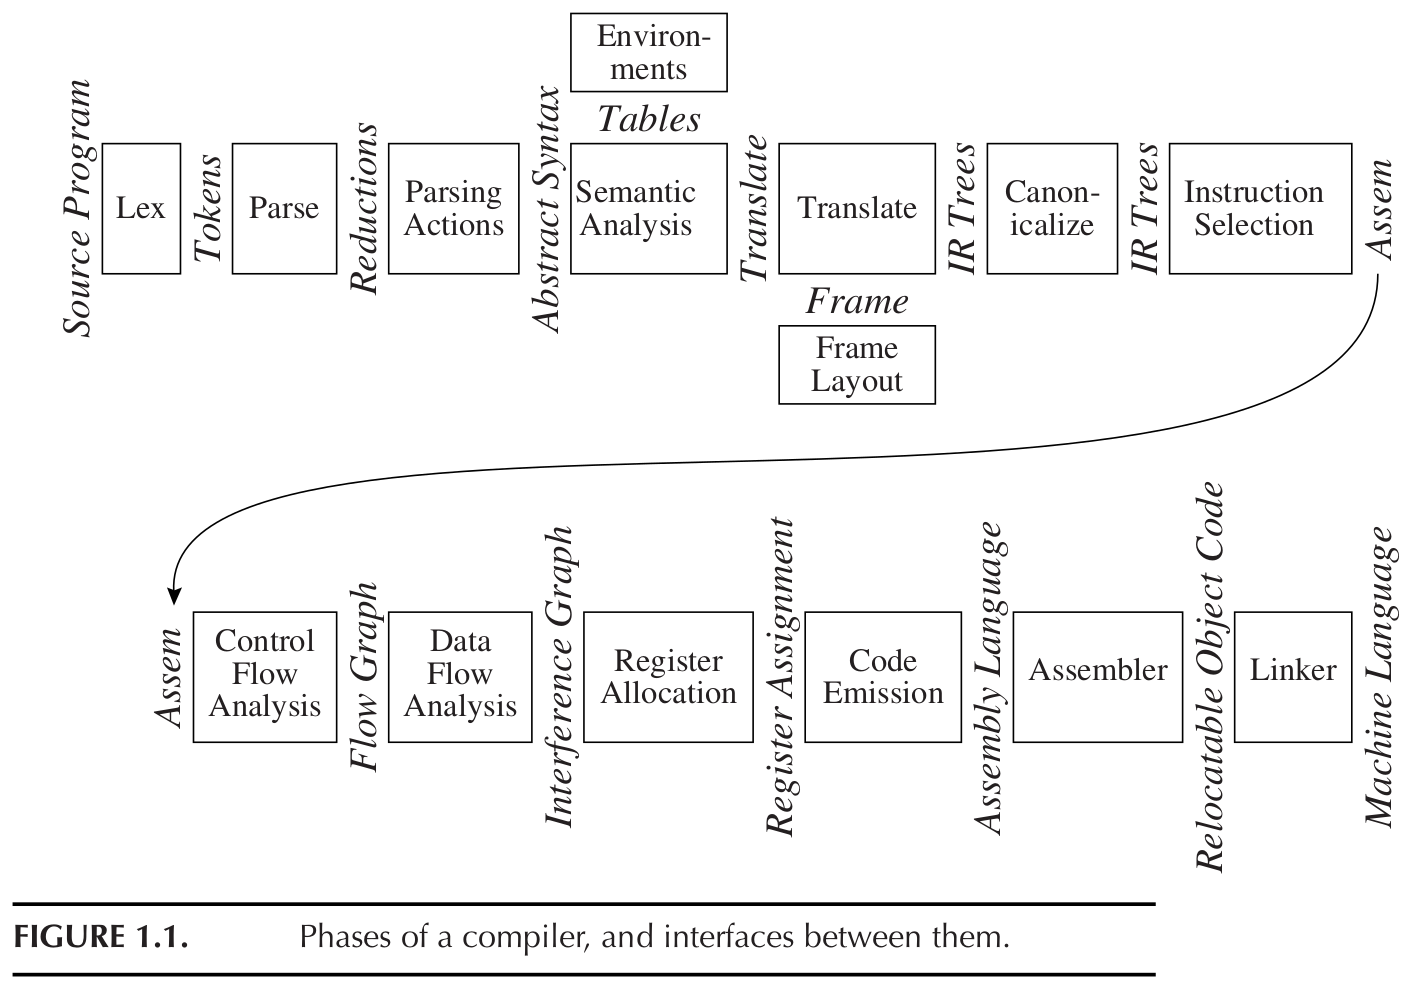
\includegraphics[width=\textwidth]{compiler_phases.png}
\end{frame}


% Vraag aan publiek de onderdelen van een stack, noteer ze op het bord om tot het schema in de volgende slide te komen
% (Denken ze aan static links voor lexical scoping? Aan guard values? Alle nodige pointers?)
\begin{frame}
    Wat zit er in een stack frame?
\end{frame}

% Vergelijk stack aan bord met stack van het handboek
% Overloop puntjes
% register allocator wordt later nog uitgelegd door Jacob
\begin{frame}{Stack van het handboek}
	\begin{columns}
	    \begin{column}{.5\textwidth}
	        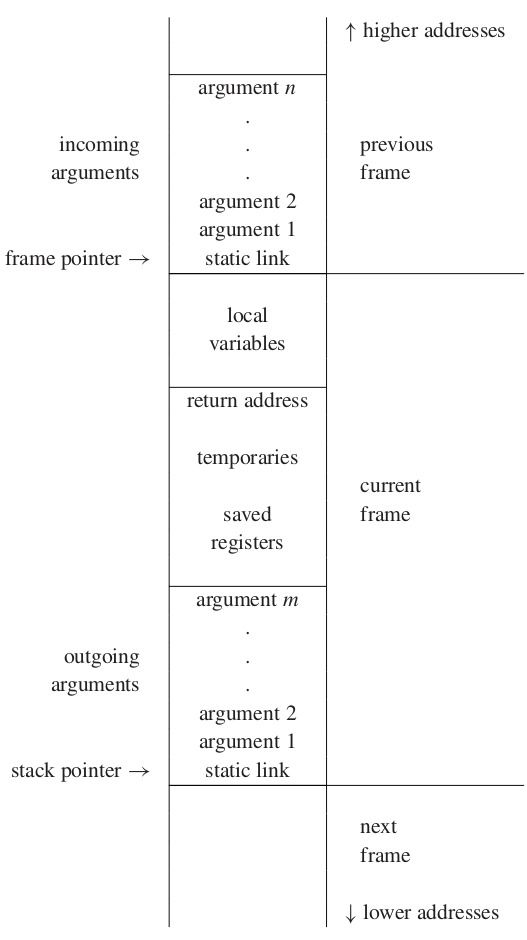
\includegraphics[height=\textheight]{theoretical_stack.png}
	    \end{column}
	    \begin{column}{.5\textwidth}
	        \begin{itemize}
	            \item Geen echte \emph{stack}
	            \item Geen \emph{echte} stack
	            \item Register allocator (zie later met Jacob)
	        \end{itemize}
	    \end{column}
	\end{columns}
\end{frame}

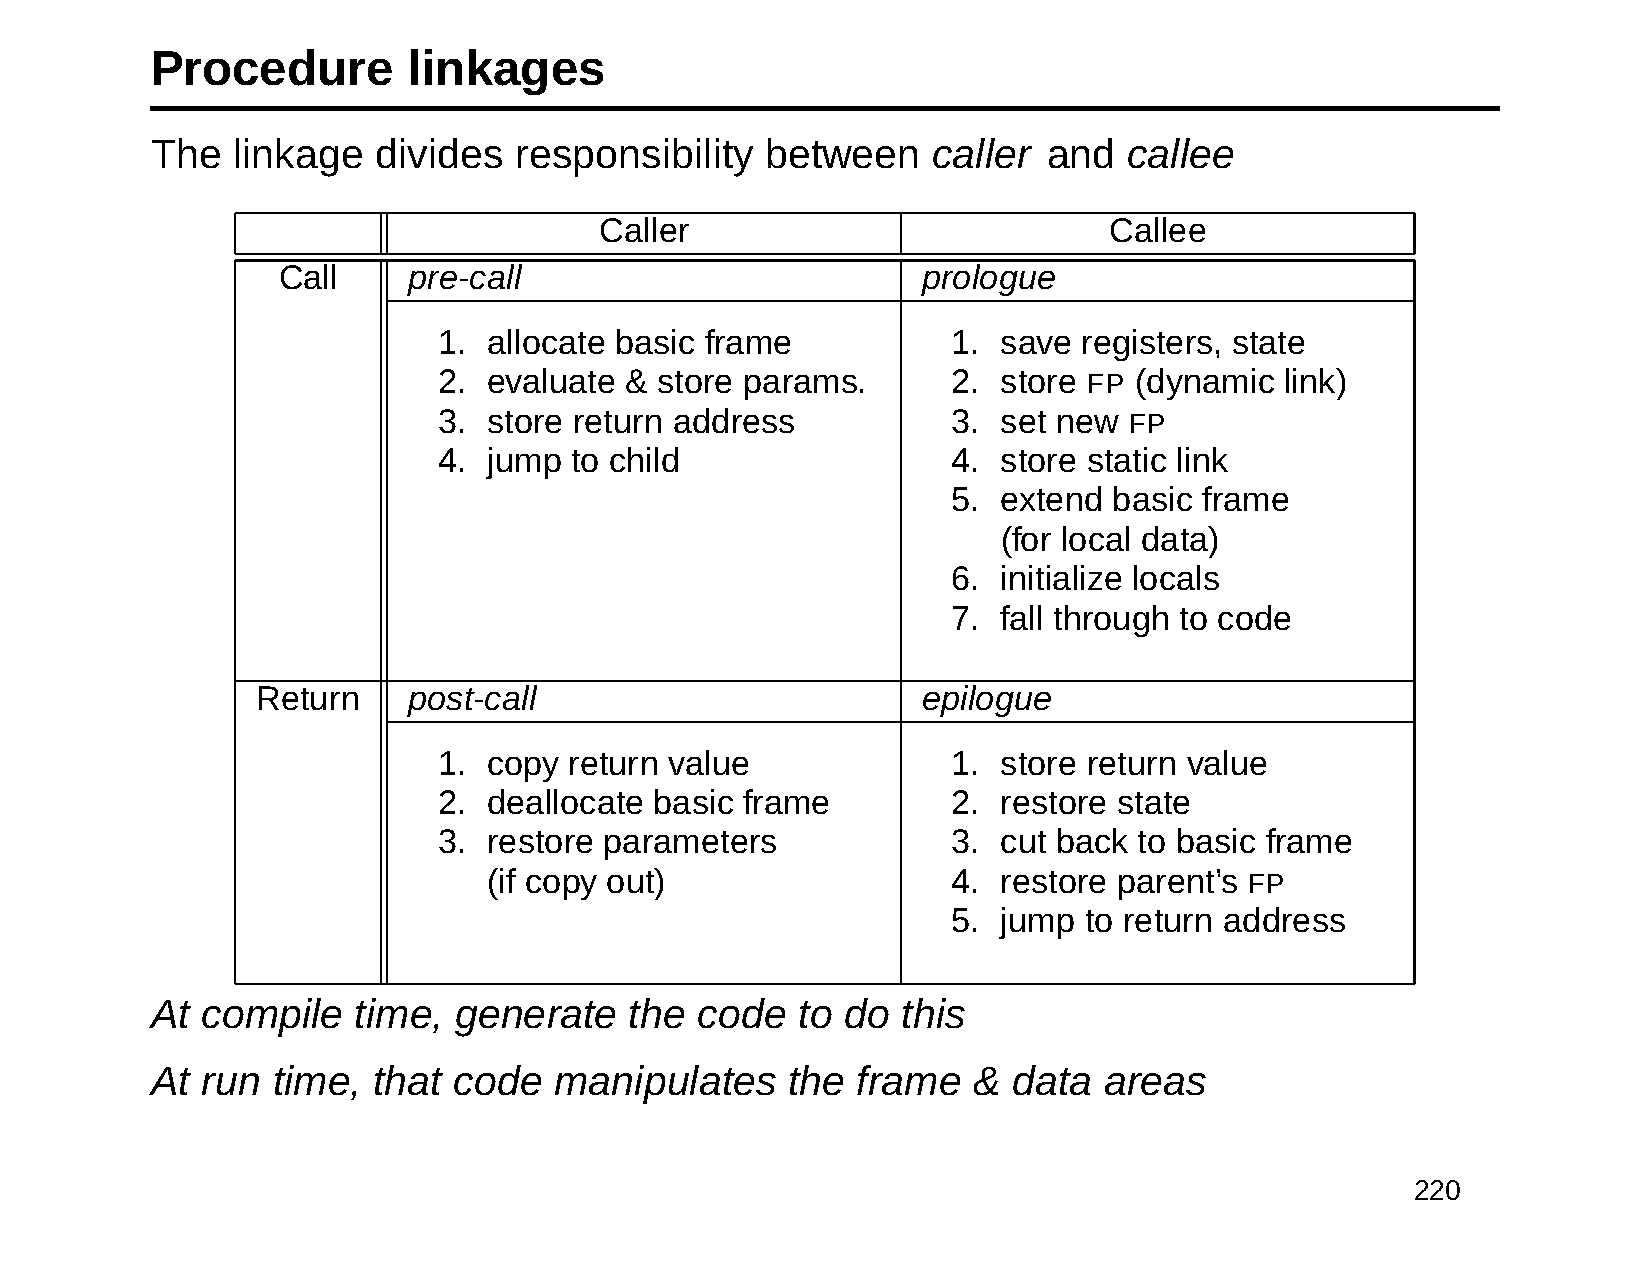
\includepdf[]{procedure_responsabilities_ucla.pdf}

\begin{frame}{Nut van een frame pointer}
	\begin{itemize}
	    \item Frames van variabele lengte (dynamic link)
	    \item Compiler kan vroeger aannames maken
	    \item Programmeur kan functies volgen in assembly
	\end{itemize}
\end{frame}

% Waarom niet alles op de stack?
\begin{frame}{Parameter passing}
Waarom geven we parameters zo veel mogelijk door via registers?
\end{frame}

\begin{frame}{Parameter passing}
	Waarom geven we parameters zo veel mogelijk door via registers?
	Snelheid!
    \begin{enumerate}
        \item leaf procedures: $l = intern * (children-1) + 1$
        \item interprocedural register allocation
        \item dead variables
        \item specific architectures (register windows)
    \end{enumerate}
\end{frame}

\begin{frame}{Calling conventions}
	\begin{itemize}
	    \item iedere taal/compiler kan kiezen
	    \item samenwerken: standaard gebruiken
	    \item stack data layout
	    \item caller-save vs callee-save
	    \item leaf functies gebruiken caller-save
	\end{itemize}
\end{frame}

\begin{frame}{ABI}
	\begin{itemize}
	    \item compiler kan verschillende ABIs ondersteunen
	    \item vb. rust
	    \item 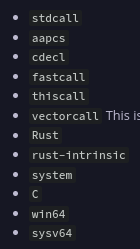
\includegraphics[width=0.3\textwidth]{abis.png}
	    \item windows 32 c: stdcall
	    \item windows 64 c: C
	\end{itemize}
\end{frame}

\begin{frame}{Tail call optimization}
	\begin{itemize}
	    \item recursieve functies
	    \item stack herbruiken
	\end{itemize}
\end{frame}

\begin{frame}{Tail call optimization}
	\begin{columns}
		\begin{column}{.4\textwidth}
		    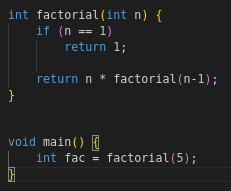
\includegraphics[width=\textwidth]{not_tco.png}
		\end{column}
		\begin{column}{.5\textwidth}
		    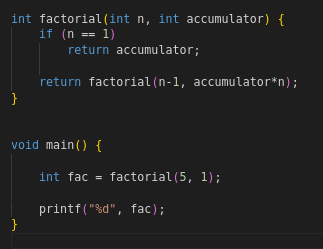
\includegraphics[width=\textwidth]{tco_2.png}
		\end{column}
	\end{columns}
\end{frame}

% overwriting stack return address or local variables
% defenses? (vanuit compiler):
%   - guard values
\begin{frame}{Stack Smashing}
	\begin{block}{What can the compiler do?}
		\begin{itemize}
		    \item Add stack canaries (terminator, random, random XOR'ed)
		    \item Add bounds checking
		\end{itemize}
	\end{block}
	Meer in de les Development of Secure Software.
\end{frame}

\begin{frame}{Demo: spelen met \texttt{gdb}}
    Examples:
    \begin{itemize}
        \item https://github.com/Toobsterrr/activation\_records.git
        \item Functie die andere functie callt
        \item Functie met veel parameters (om spilling van de registers te demonstreren)
        \item Functie die waardes returnt
        \item Functie die via een buffer de stack manipuleert
        % \item Functie die stack overschrijft (hack hehe)
        \item Verschillende optimization levels testen
        \item Tail call optimization
    \end{itemize}
\end{frame}

\begin{frame}{Nested functions}
    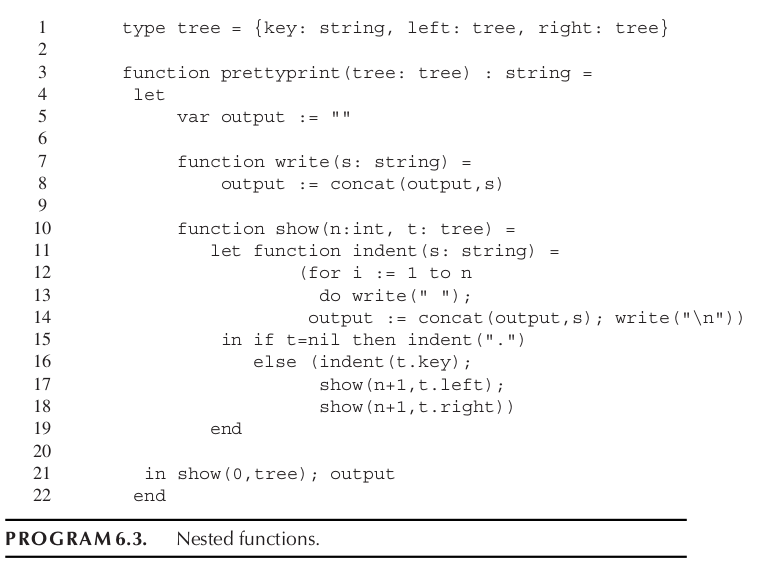
\includegraphics[width=\textwidth]{nested_functions.png}
\end{frame}

\begin{frame}{Nested functions: solutions}
    \begin{itemize}
        \item Static links
        \item Display
        \item Lambda lifting
    \end{itemize}
\end{frame}

% Voorbeeld uit het boek
\begin{frame}{Wanneer is een stack niet genoeg?}
	\begin{block}{}
	    Nested functions \&\& Functions as return values
	\end{block}
	\begin{block}{Oplossing}
	    Heap-allocation en garbage collection
	\end{block}
\end{frame}

\begin{frame}{Continuations}
	\begin{block}{Definitie}
	    A continuation is the abstract concept represented by the control stack, or dynamic chain of activation records, in a typical programming-language implementation.
	\end{block}
	\begin{itemize}
	    \item Zoals closures environments opslaan, zo slaan continuations de huidige controlecontext op (de stack)
	    \item Gelijkenissen met multithreading
	    \item Kan gebruikt worden om try-catch structuren te maken
	\end{itemize}
\end{frame}

\begin{frame}{Continuations: implementatie}
	\begin{itemize}
	    \item The garbage-collection strategy
	    \item The spaghetti stack
	\end{itemize}
\end{frame}

\begin{frame}{Examenvragen}
    \begin{itemize}
        \item Leg uit hoe de stack verandert wanneer een nieuwe procedure wordt opgeroepen.
        \item Leg uit hoe het doorgeven van parameters via de registers zorgt voor efficiënter geheugengebruik.
        \item Leg tail call optimization uit en pas het toe op een voorbeeldprogramma.
        \item Gegeven een voorbeeldprogramma, kan dit programma activation records gebruiken die toegewezen zijn op een stack? Waarom?
    \end{itemize}
\end{frame}

\begin{frame}{Extra source}
	\begin{itemize}
	    \item Laatste hoofdstuk van deze slides: \href{https://web.cs.ucla.edu/~palsberg/course/cs132/lec.pdf}{https://web.cs.ucla.edu/~palsberg/course/cs132/lec.pdf}
	    \item \emph{Implementation strategies for First-Class Continuations} van William D. Clinger (voor de geïnteresseerden)
	\end{itemize}
\end{frame}

\end{document}

